\hypertarget{day-7---ux7f16ux5199-mvc}{%
\subsection{Day 7 - 编写 MVC}\label{day-7---ux7f16ux5199-mvc}}

现在,ORM 框架、Web 框架和配置都已就绪,我们可以开始编写一个最简单的
MVC,把它们全部启动起来。

通过 Web 框架的\texttt{@get}和 ORM 框架的 Model
支持,可以很容易地编写一个处理首页 URL 的函数:

\begin{pythoncode}
@get('/')
def index(request):
    users = yield from User.findAll()
    return {
        '__template__': 'test.html',
        'users': users
    }
\end{pythoncode}

\texttt{\textquotesingle{}\_\_template\_\_\textquotesingle{}}指定的模板文件是\texttt{test.html},其他参数是传递给模板的数据,所以我们在模板的根目录\texttt{templates}下创建\texttt{test.html}:

\begin{pythoncode}
<!DOCTYPE html>
<html>
<head>
    <meta charset="utf-8" />
    <title>Test users - Awesome Python Webapp</title>
</head>
<body>
    <h1>All users</h1>
    
    <p>{{ u.name }} / {{ u.email }}</p>
    
</body>
</html>
\end{pythoncode}

接下来,如果一切顺利,可以用命令行启动 Web 服务器:

\begin{pythoncode}
$ python3 app.py
\end{pythoncode}

然后,在浏览器中访问\texttt{http://localhost:9000/}。

如果数据库的\texttt{users}表什么内容也没有,你就无法在浏览器中看到循环输出的内容。可以自己在
MySQL 的命令行里给\texttt{users}表添加几条记录,然后再访问:

 
 \begin{figure}[htp]
	\centering
	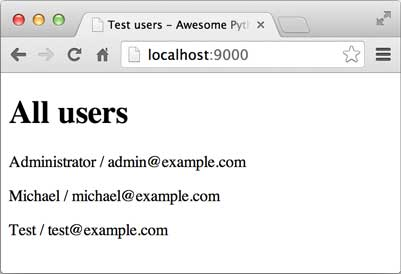
\includegraphics[width=0.6\linewidth]{fig/955624199250624.png}
\end{figure}


\hypertarget{ux53c2ux8003ux6e90ux7801}{%
\subsubsection{参考源码}\label{ux53c2ux8003ux6e90ux7801}}

\href{https://github.com/michaelliao/awesome-python3-webapp/tree/day-07}{day-07}

